\documentclass[12pt]{article}
\author{Lawrence Liu}
\usepackage{subcaption}
\usepackage{graphicx}
\usepackage{amsmath}
\usepackage{pdfpages}
\newcommand{\Laplace}{\mathscr{L}}
\setlength{\parskip}{\baselineskip}%
\setlength{\parindent}{0pt}%
\usepackage{xcolor}
\usepackage{listings}
%\definecolor{backcolour}{rgb}{0.95,0.95,0.92}
\usepackage{amssymb}
\usepackage[T1]{fontenc}
\usepackage{beramono}%\lstdefinestyle{mystyle}{
%    backgroundcolor=\color{backcolour}}
%\lstset{style=mystyle}
%\usepackage[usenames,dvipsnames]{xcolor}%%
%% Julia definition (c) 2014 Jubobs
%%



\title{ECE 133A HW 6}
\begin{document}
\maketitle
\section*{Exercise A9.4}
Since $A=T(B)$, $D_v=T(E)$, and $D_h=T(E^T)$, and letting
$b$, $e$, and $f$ being the column major ordering of $B$, $E$ and  
We have that $A$, $D_v$, and $D_h$ are all real matrices.  Thus,
we have
$$A^T=A^H=\frac{1}{n^2}\tilde{W}\textbf{diag}(\overline{\tilde{W}b})\tilde{W}^H$$
Where $\circ$ denotes element wise multiplication, the same can be done for $D_v^T$ and $D_h^T$. Thus we have that
$$A^TA=\frac{1}{n^2}\tilde{W}\textbf{diag}\left(\tilde{W}b\circ\overline{\tilde{W}b}\right)\tilde{W}^Hx$$
And likewise for $D_v^TD_v$ and $D_h^TD_h$. Thus we have that
$$(A^TA+\lambda D^T_vD_v+\lambda D^T_hD_h)x=A^Ty$$
becomes:
\begin{align*}
    \frac{1}{n^2}\tilde{W}\left(\textbf{diag}\left(\tilde{W}b\circ\overline{\tilde{W}b}\right) +\lambda \textbf{diag}\left(\tilde{W}e\circ\overline{\tilde{W}e}\right) 
            +\lambda \textbf{diag}\left(\tilde{W}f\circ\overline{\tilde{W}f}\right)\right)\tilde{W}^Hx
            &=\frac{1}{n^2}\tilde{W}\textbf{diag}(\tilde{W}b)\tilde{W}^Hy\\
            \frac{1}{n^2}\left(\textbf{diag}\left(\tilde{W}b\circ\overline{\tilde{W}b}\right) +\lambda \textbf{diag}\left(\tilde{W}e\circ\overline{\tilde{W}e}\right) 
            +\lambda \textbf{diag}\left(\tilde{W}f\circ\overline{\tilde{W}f}\right)\right)\tilde{W}^Hx
            &=\frac{1}{n^2}\textbf{diag}(\tilde{W}b)\tilde{W}^Hy
\end{align*}
let $z=\frac{1}{n^2}\tilde{W}^Hx$ Then we get
$$\left(\textbf{diag}\left(\tilde{W}b\circ\overline{\tilde{W}b}\right) +\lambda \textbf{diag}\left(\tilde{W}e\circ\overline{\tilde{W}e}\right) 
            +\lambda \textbf{diag}\left(\tilde{W}f\circ\overline{\tilde{W}f}\right)\right)z
            =\frac{1}{n^2}\textbf{diag}(\tilde{W}b)\tilde{W}^Hy$$
Then solving for $\tilde{W}b$, $\tilde{W}e$, and $\tilde{W}f$ and $\frac{1}{n^2}\tilde{W}^Hy$ 
will cost $n^2\log(n)$ flops each, and then solving for 
$\left(\textbf{diag}\left(\tilde{W}b\circ\overline{\tilde{W}b}\right) +\lambda \textbf{diag}\left(\tilde{W}e\circ\overline{\tilde{W}e}\right) 
+\lambda \textbf{diag}\left(\tilde{W}f\circ\overline{\tilde{W}f}\right)\right)$ will cost 
us $10n$ flops. Likewise solving for $\frac{1}{n^2}\textbf{diag}(\tilde{W}b)\tilde{W}^Hy$
is just element wise multiplication of $\frac{1}{n^2}\tilde{W}^Hy$ and 
$\tilde{W}b$ which is $n^2$ flops. Then we can solve for 
$z$ by dividing $\frac{1}{n^2}\textbf{diag}(\tilde{W}b)\tilde{W}^Hy$
by $\left(\textbf{diag}\left(\tilde{W}b\circ\overline{\tilde{W}b}\right) +\lambda \textbf{diag}\left(\tilde{W}e\circ\overline{\tilde{W}e}\right)
+\lambda \textbf{diag}\left(\tilde{W}f\circ\overline{\tilde{W}f}\right)\right)$
element wise which will cost us $n^2$ flops. Then we can solve for $x$ by 
just multiplying $z$ with $\tilde{W}$ 
or in other words, dong the FFT on $z$, which will cost us $n^2\log(n)$ flops. 
Therefore in total our algorithm will cost us 
$5n^2\log(n)+12n^2$ flops. This can be implemented with the 
following algorithm
\begin{verbatim}
function x=deblur(Y,B,lambda)
    %convert Y to column major order
    y = Y(:);
    %convert B to column major order
    b = B(:);
    %make the E matrix where all values are 0 except for 
    %the top left bottom left values
    %which are 1 and -1 respectively
    E=zeros(size(B));
    E(1,1)=1;
    E(end,1)=-1;
    %convert E to column major order
    e = E(:);
    %convert the transpose of E to column major order
    f = E'(:);
    
    n=size(B,1);

    fft_b=reshape( fft2( reshape( b, n, n ) ), n^2, 1);
    fft_e=reshape( fft2( reshape( e, n, n ) ), n^2, 1);
    fft_f=reshape( fft2( reshape( f, n, n ) ), n^2, 1);
    ifft_y=reshape( ifft2( reshape( y, n, n ) ), n^2, 1);

    z=(fft_b.*ifft_y)./(fft_b.*conj(fft_b)+
            lambda*(fft_e.*conj(fft_e)+fft_f.*conj(fft_f)));
    x=reshape( fft2( reshape( z, n, n ) ), n^2, 1);
end
\end{verbatim}
\subsection*{(b)}
With the function above and the code below, I generated the following
deblurred images for different values of $\lambda$.
\begin{verbatim}
load HW6/deblur.mat
gcf=figure;
Lambdas=10.^(-6:-2);
x0=10;
y0=10;
width=500*2;
height=500*(length(Lambdas)+1)/2;
set(gcf,'position',[x0,y0,width,height])
subplot((length(Lambdas)+1)/2,2,1)
imshow(Y,[])
title('Original Image');
hold on
for i=1:length(Lambdas)
    i
    subplot((length(Lambdas)+1)/2,2,i+1);
    lambda=Lambdas(i)
    x=deblur(Y,B,lambda);
    imshow(reshape(x,1024,1024),[]);
    title(sprintf('lambda=%f',lambda));
end
print -dpng problem1.png
hold off
\end{verbatim}
To get the following images\\
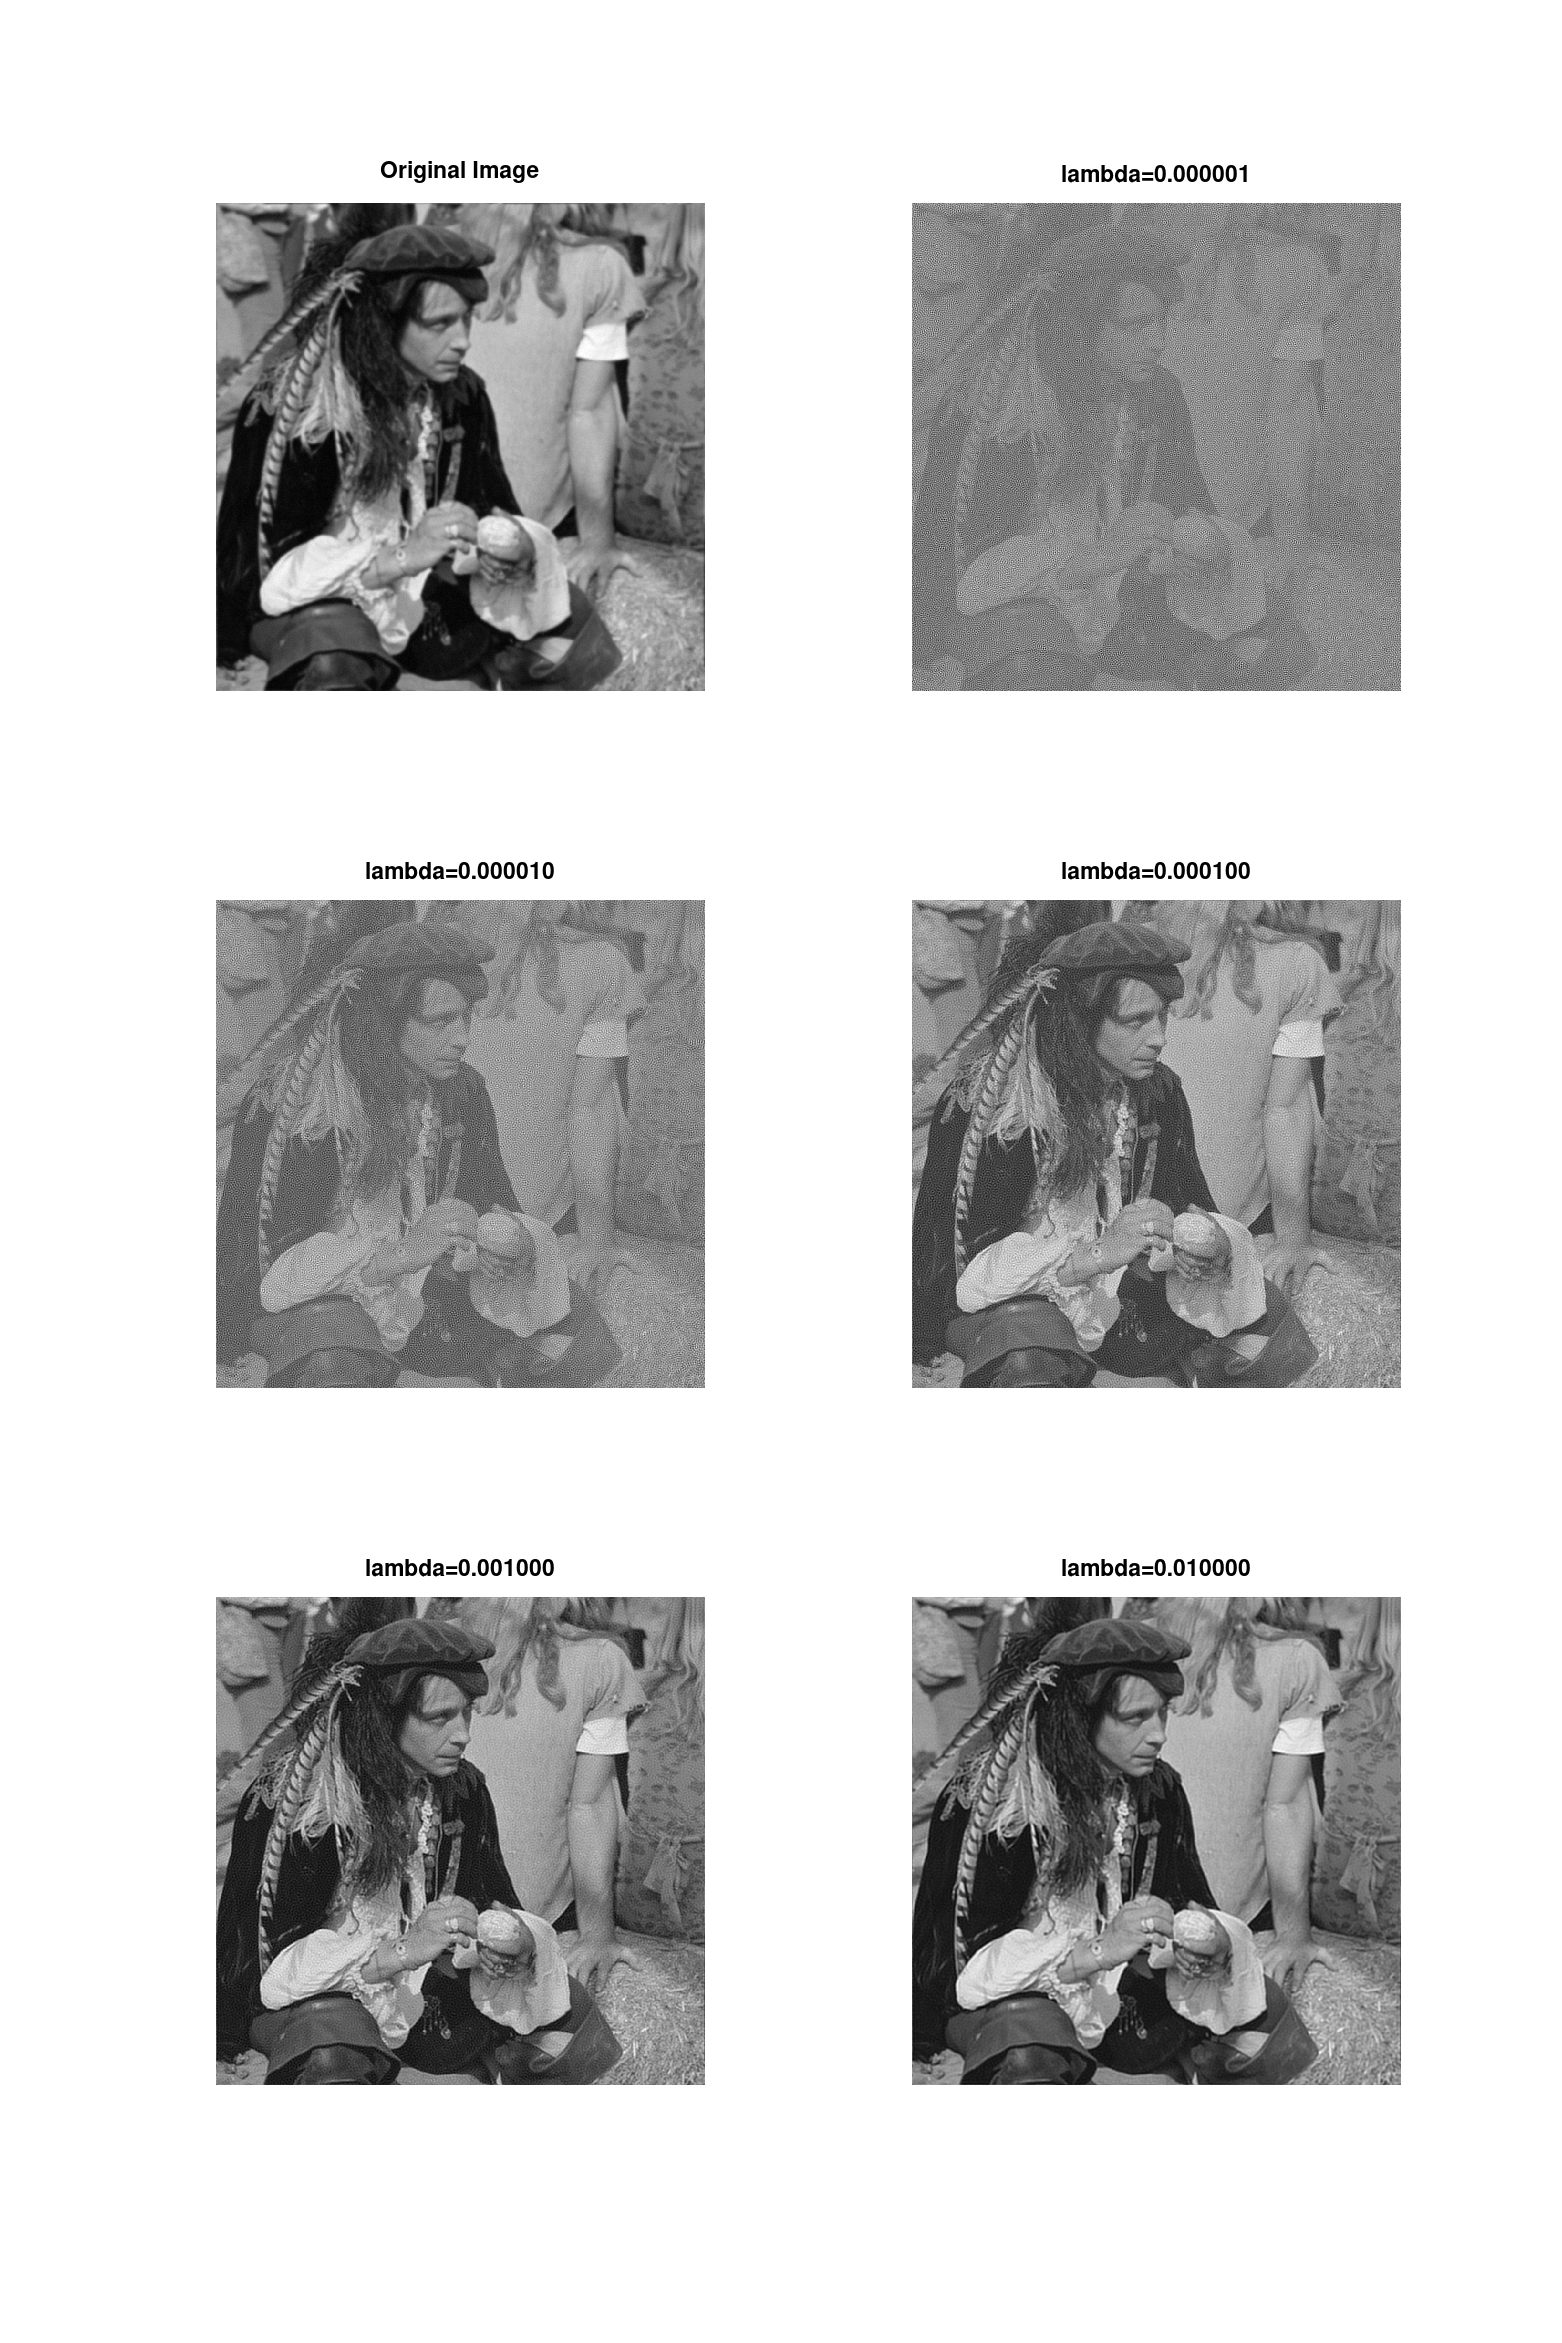
\includegraphics[scale=0.25]{problem1.png}\\
Visually it seems like $\lambda =10^{-3}$ produces the best debluring.
\section*{Exercise A10.1}
\subsection*{(a)}
Let $u=[u(0),u(1),\cdots,u(N-1)]^T$, then we have that $x=u$
we want to minimize the energy or 
$$||u||^2$$
Furthermore we can express 
$$s_1(N)=0.1u(N-2)+(0.95+1)\cdot 0.1 u(N-3)+(0.95^2+0.95+1)\cdot 0.1 u(N-4)+\cdots+(\sum_{i=0}^{N-2}0.95^i)\cdot 0.1 u(0)$$
$$s_2(N)=0.1u(N-1)+(0.95)\cdot 0.1 u(N-2)+(0.95^2)\cdot 0.1 u(N-3)+\cdots+(0.95^{N-1})\cdot 0.1 u(0)$$
So therefore we have that 
$$C=\begin{bmatrix}
    0.1\sum_{i=0}^{N-2}0.95^i & \cdots & 0.1(0.95+1) & 0.1 & 0\\
    0.1(0.95^{N-1}) & \cdots & 0.1(0.95^2) &  0.1(0.95) & 0.1
\end{bmatrix}$$
And
$$d=\begin{bmatrix}
    10\\
    0
\end{bmatrix}$$
\subsection*{(b)}
\begin{verbatim}
using PyPlot

function create_C(N)
    C = zeros(2,N)

    #make the first row of C 
    for i=1:N-1
        for j=1:N-i
            C[1,i]+=0.1*(0.95^(j-1))
        end
    end
    # C[1,N-1]=0.1 

    #make the second row of C 
    for i=1:N
        C[2,i] = 0.1*(0.95^(N-i))
    end
    return C
end

# calculate u
N=30
C = create_C(N)
d=[10,0]
u = C\d
s1=zeros(N+1)
s2=zeros(N+1)
for i=1:N
    s1[i+1]=s1[i]+s2[i]
    s2[i+1]=0.95*s2[i]+0.1*u[i]
end

fig,axs=subplots(3,1,figsize=(10,12))
axs[1].plot(s1)
axs[1][:set_title]("s1")
axs[2][:plot](s2)
axs[2][:set_title]("s2")
axs[3][:plot](u)
axs[3][:set_title]("u")
axs[3][:set_xlabel]("time")

savefig("problem2a.png")
close()
\end{verbatim}
We get the following plot\\
\includegraphics*[scale=0.4]{problem2a.png}
\subsection*{(c)}
With the following code:
\begin{verbatim}
using PyPlot

function create_C(N)
    C = zeros(2,N)

    #make the first row of C 
    for i=1:N-1
        for j=1:N-i
            C[1,i]+=0.1*(0.95^(j-1))
        end
    end
    # C[1,N-1]=0.1 

    #make the second row of C 
    for i=1:N
        C[2,i] = 0.1*(0.95^(N-i))
    end
    return C
end

N=2:29
println(N)
E=zeros(length(N))
for i=1:length(N)
    C = create_C(N[i])
    d=[10,0]
    u = C\d
    E[i]=sum(u.^2)
end
plot(N,E)
xlabel("N")
ylabel("E")
yscale("log")
savefig("problem2b.png")
close()
\end{verbatim}
We get the following plot\\
\includegraphics*[scale=0.7]{problem2b.png}
\section*{Exercise A10.9}
\subsection*{(a)}
We use Langrage multipliers to solve this problem.\\
$$L(x)=||Ax-b||^2+\lambda e_i^T x$$
\begin{align*}
    \nabla L(x)&=0\\
    2A^T(Ax-b)+\lambda e_i&=0\\
    2A^TAx&=2A^Tb-\lambda e_i\\
    A^TAx&=A^Tb-\frac{\lambda}{2} e_i\\
    x&=(A^TA)^{-1}A^Tb-\frac{\lambda}{2}(A^TA)^{-1}e_i\\
    x&=\hat{x}-\frac{\lambda}{2}(A^TA)^{-1}e_i
\end{align*}
subsituting this back into the constraint we get
\begin{align*}
    e_i^T x&=0\\
    e_i^T\left(\hat{x}-\frac{\lambda}{2}(A^TA)^{-1}e_i\right)&=0\\
    \hat{x}_i-\frac{\lambda}{2}(A^TA)^{-1}_{ii}&=0\\
    \hat{x}_i&=\frac{\lambda}{2}(A^TA)^{-1}_{ii}
    \lambda=\frac{2\hat{x}_i}{(A^TA)^{-1}_{ii}}
\end{align*}
And thus we get that
$$x=\hat{x}-\frac{\hat{x}_i}{(A^TA)^{-1}_{ii}}(A^TA)^{-1}e_i$$
\subsection*{(b)}
Calculating the QR factorization of A costs $2mn^2$ flops. 
And solving $\hat{x}$ costs an additional $2mn+n^2$ flops.
Then we can solve for $(A^TA)^{-1}e_i$ using 
backwards and forwards substitution which costs $2n^2$ flops, and 
then finding $(A^TA)^{-1}_{ii}$ is just finding the value
for the ith index in the vector $(A^TA)^{-1}e_i$ which costs $0$ flops.
This is the same for $\hat{x}_i$. Then calculating 
$\frac{\hat{x}_i}{(A^TA)^{-1}_{ii}}$ costs $1$ flops, and then multiplying
that to every value of $(A^TA)^{-1}e_i$ costs $n$ flops. And then subtracting the resulting
vector from $\hat{x}$ will cost $n$ flops. So the total cost is
$\boxed{2mn^2+2mn+3n^2+2n+1}$ flops.
\end{document}